\documentclass[12pt]{scrartcl}

\usepackage{amsmath,amssymb}
\usepackage{fullpage}
\usepackage{enumitem}
\usepackage{hyperref}
\usepackage{tikz}

\setlength{\parindent}{0pt}

\begin{document}

\begin{center}
	\hrule
	\vspace{0.4cm}
	{\textbf{\large INF1003 Tutorial 8}}\\[0.2cm]
\end{center}

\textbf{Name:} Timothy Chia\hspace{\fill} \textbf{Topic:} Sets\\
\textbf{Student ID:} 2501530 \hspace{\fill} \textbf{Due Date:} 2/11/2025, 10:00 PM\\

\hrule

\begin{enumerate}[label=\textbf{\arabic*.}]

	%------------------------------------------------------------
	\item List the members of the following sets.

	      \begin{enumerate}[label=(\alph*)]
		      \item $\{x \mid x \text{ is a real number such that } x^{2} = 1\}$.

		            \textbf{Solution.}
		            Solve $x^{2} = 1$ over the real numbers:
		            \[
			            x^{2} = 1 \quad\Rightarrow\quad x = \pm 1.
		            \]
		            So the set is
		            \[
			            \{-1, 1\}.
		            \]

		      \item $\{x \mid x \text{ is the cube of a positive integer such that } x \le 1728\}$.

		            \textbf{Solution.}
		            Let $x = k^{3}$ where $k$ is a positive integer and $k^{3} \le 1728$.
		            Note that $1728 = 12^{3}$, and $13^{3} = 2197 > 1728$.
		            Hence $k$ can be any integer from $1$ to $12$.
		            Thus the set of cubes is
		            \[
			            \{1, 8, 27, 64, 125, 216, 343, 512, 729, 1000, 1331, 1728\}.
		            \]

		      \item $\{x \mid x \text{ is a prime number such that } x < 15\}$.

		            \textbf{Solution.}
		            The positive integers less than $15$ are $2,3,4,\dots,14$.
		            The primes among them are $2,3,5,7,11,13$.
		            So the set is
		            \[
			            \{2, 3, 5, 7, 11, 13\}.
		            \]

		      \item $\{x \mid x \text{ is an integer such that } x^{2} = 5\}$.

		            \textbf{Solution.}
		            If $x$ is an integer and $x^{2} = 5$, then $x = \pm\sqrt{5}$,
		            but $\sqrt{5}$ is not an integer.
		            Hence there is no integer solution, so the set is empty:
		            \[
			            \emptyset.
		            \]
	      \end{enumerate}

	      %------------------------------------------------------------
	\item Suppose that $A = \{2,4,6\}$, $B = \{2,6\}$, $C = \{6,4\}$, $D = \{4,2,6\}$ and
	      $E = \{4,8,6\}$. Determine which of these sets are proper subsets of which other sets.
	      Also list the members of the following.

	      \begin{enumerate}[label=(\alph*)]
		      \item \emph{Proper subsets.}

		            \textbf{Solution.}
		            \begin{itemize}
			            \item $B = \{2,6\}$ and $A = \{2,4,6\}$, so every element of $B$ is in $A$, but $A$ has $4$ as an extra element.
			                  Thus $B \subset A$ (proper subset).
			            \item $D = \{4,2,6\}$ has exactly the same elements as $A$. So $A = D$.
			                  Therefore $B \subset D$ as well.
			            \item $C = \{6,4\}$; this is a subset of $A$ (and $D$) and also of $E$:
			                  \[
				                  C \subset A,\quad C \subset D,\quad C \subset E.
			                  \]
			            \item No other non-trivial proper subset relations hold (for instance, $E$ is not a subset of $A$ because $8 \in E$ but $8 \notin A$).
		            \end{itemize}

		      \item $A \cap C$.

		            \textbf{Solution.}
		            \[
			            A \cap C = \{2,4,6\} \cap \{6,4\} = \{4,6\}.
		            \]

		      \item $B \cup E$.

		            \textbf{Solution.}
		            \[
			            B \cup E = \{2,6\} \cup \{4,8,6\} = \{2,4,6,8\}.
		            \]

		      \item $D \cap B \cap E$.

		            \textbf{Solution.}
		            First compute $D \cap B$:
		            \[
			            D \cap B = \{4,2,6\} \cap \{2,6\} = \{2,6\}.
		            \]
		            Then intersect with $E$:
		            \[
			            (D \cap B) \cap E = \{2,6\} \cap \{4,8,6\} = \{6\}.
		            \]
		            So $D \cap B \cap E = \{6\}$.
	      \end{enumerate}

	      %------------------------------------------------------------
	\item What is the cardinality of each of these sets?

	      \begin{enumerate}[label=(\alph*)]
		      \item $\{a\}$

		            \textbf{Solution.}
		            There is exactly one element, namely $a$, so
		            \[
			            |\{a\}| = 1.
		            \]

		      \item $\{\{a\}\}$

		            \textbf{Solution.}
		            Here the single element of the set is the set $\{a\}$.
		            So there is still exactly one element:
		            \[
			            |\{\{a\}\}| = 1.
		            \]

		      \item $\{a,\{a\}\}$

		            \textbf{Solution.}
		            The elements are $a$ and the set $\{a\}$, which are distinct objects.
		            Hence there are two elements:
		            \[
			            |\{a,\{a\}\}| = 2.
		            \]

		      \item $\{a,\{a\},\{a,\{a\}\}\}$

		            \textbf{Solution.}
		            The elements are $a$, the set $\{a\}$, and the set $\{a,\{a\}\}$, all distinct.
		            So there are three elements:
		            \[
			            \bigl|\{a,\{a\},\{a,\{a\}\}\}\bigr| = 3.
		            \]

		      \item $\emptyset$

		            \textbf{Solution.}
		            The empty set has no elements, so
		            \[
			            |\emptyset| = 0.
		            \]

		      \item $\{\emptyset\}$

		            \textbf{Solution.}
		            This set has a single element, namely the empty set. Thus
		            \[
			            |\{\emptyset\}| = 1.
		            \]

		      \item $\{\emptyset,\{\emptyset\}\}$

		            \textbf{Solution.}
		            The two elements are $\emptyset$ and the set $\{\emptyset\}$, which are distinct.
		            Therefore
		            \[
			            \bigl|\{\emptyset,\{\emptyset\}\}\bigr| = 2.
		            \]

		      \item $\{\emptyset,\{\emptyset\},\{\emptyset,\{\emptyset\}\}\}$

		            \textbf{Solution.}
		            The three elements are $\emptyset$, $\{\emptyset\}$, and $\{\emptyset,\{\emptyset\}\}$,
		            all distinct, so
		            \[
			            \bigl|\{\emptyset,\{\emptyset\},\{\emptyset,\{\emptyset\}\}\}\bigr| = 3.
		            \]
	      \end{enumerate}

	      %------------------------------------------------------------
	\item List the elements of the following sets, where $a$ and $b$ are distinct elements, and $P(\cdot)$
	      denotes the power set.

	      \begin{enumerate}[label=(\alph*)]
		      \item $P(\{a,b\})$.

		            \textbf{Solution.}
		            All subsets of $\{a,b\}$ are
		            \[
			            \emptyset,\quad \{a\},\quad \{b\},\quad \{a,b\}.
		            \]
		            Hence
		            \[
			            P(\{a,b\}) = \{\emptyset,\{a\},\{b\},\{a,b\}\}.
		            \]

		      \item $P(\{a,\emptyset\})$.

		            \textbf{Solution.}
		            Now the two elements are $a$ and $\emptyset$.
		            Subsets:
		            \[
			            \emptyset,\quad \{a\},\quad \{\emptyset\},\quad \{a,\emptyset\}.
		            \]
		            So
		            \[
			            P(\{a,\emptyset\}) = \{\emptyset,\{a\},\{\emptyset\},\{a,\emptyset\}\}.
		            \]

		      \item $P(\{a,\{\emptyset\}\})$.

		            \textbf{Solution.}
		            The elements are $a$ and the set $\{\emptyset\}$.
		            Subsets:
		            \[
			            \emptyset,\quad \{a\},\quad \{\{\emptyset\}\},\quad \{a,\{\emptyset\}\}.
		            \]
		            Hence
		            \[
			            P(\{a,\{\emptyset\}\}) =
			            \{\emptyset,\{a\},\{\{\emptyset\}\},\{a,\{\emptyset\}\}\}.
		            \]

		      \item $P(\{a,b,\{a,b\}\})$.

		            \textbf{Solution.}
		            This set has three elements: $a$, $b$, and $\{a,b\}$.
		            A $3$-element set has $2^{3}=8$ subsets:
		            \[
			            \emptyset,\;
			            \{a\},\;
			            \{b\},\;
			            \{\{a,b\}\},\;
			            \{a,b\},\;
			            \{a,\{a,b\}\},\;
			            \{b,\{a,b\}\},\;
			            \{a,b,\{a,b\}\}.
		            \]
		            So
		            \[
			            P(\{a,b,\{a,b\}\}) =
			            \{\emptyset,\{a\},\{b\},\{\{a,b\}\},\{a,b\},\{a,\{a,b\}\},\{b,\{a,b\}\},
			            \{a,b,\{a,b\}\}\}.
		            \]

		      \item $P(P(\emptyset))$.

		            \textbf{Solution.}
		            First $P(\emptyset) = \{\emptyset\}$.
		            Then $P(\{\emptyset\})$ has subsets
		            \[
			            \emptyset \quad\text{and}\quad \{\emptyset\}.
		            \]
		            Hence
		            \[
			            P(P(\emptyset)) = \{\emptyset,\{\emptyset\}\}.
		            \]
	      \end{enumerate}

	      %------------------------------------------------------------
	\item Let $A=\{a,b,c,d\}$ and $B=\{y,z\}$. Find

	      \begin{enumerate}[label=(\alph*)]
		      \item $A \times B$;

		            \textbf{Solution.}
		            By definition,
		            \[
			            A \times B = \{(x,y) \mid x \in A, y \in B\}.
		            \]
		            So we pair each element of $A$ with each element of $B$:
		            \[
			            A \times B =
			            \{(a,y),(a,z),(b,y),(b,z),(c,y),(c,z),(d,y),(d,z)\}.
		            \]

		      \item $B \times A$.

		            \textbf{Solution.}
		            Now
		            \[
			            B \times A =
			            \{(y,a),(y,b),(y,c),(y,d),(z,a),(z,b),(z,c),(z,d)\}.
		            \]
	      \end{enumerate}

	      %------------------------------------------------------------
	\item Let the universal set $U = \{0,1,2,3,4,5,6,7,8,9,10\}$, and let
	      \[
		      A = \{0,2,4,6,8,10\},\quad
		      B = \{0,1,2,3,4,5,6\},\quad
		      C = \{4,5,6,7,8,9,10\}.
	      \]
	      For each set below, list the members and draw the corresponding Venn diagram.

	      \begin{enumerate}[label=(\alph*)]
		      \item $A \cap B \cap C$.

		            \textbf{Solution.}
		            First,
		            \[
			            A \cap B = \{0,2,4,6\},
		            \]
		            then
		            \[
			            (A \cap B) \cap C = \{0,2,4,6\} \cap \{4,5,6,7,8,9,10\} = \{4,6\}.
		            \]
		            So $A \cap B \cap C = \{4,6\}$.

		      \item $A \cup B \cup C$.

		            \textbf{Solution.}
		            \[
			            A \cup B = \{0,1,2,3,4,5,6,8,10\},
		            \]
		            and
		            \[
			            (A \cup B) \cup C = \{0,1,2,3,4,5,6,8,10\} \cup \{4,5,6,7,8,9,10\}
			            = \{0,1,2,3,4,5,6,7,8,9,10\} = U.
		            \]
		            So $A \cup B \cup C = U$.

		      \item $(A \cup B) \cap C$.

		            \textbf{Solution.}
		            From above, $A \cup B = \{0,1,2,3,4,5,6,8,10\}$. Then
		            \[
			            (A \cup B) \cap C =
			            \{0,1,2,3,4,5,6,8,10\} \cap \{4,5,6,7,8,9,10\}
			            = \{4,5,6,8,10\}.
		            \]

		      \item $(A \cap B) \cup C$.

		            \textbf{Solution.}
		            We have $A \cap B = \{0,2,4,6\}$, hence
		            \[
			            (A \cap B) \cup C =
			            \{0,2,4,6\} \cup \{4,5,6,7,8,9,10\}
			            = \{0,2,4,5,6,7,8,9,10\}.
		            \]

		      \item $(A \cup (B \cap C))^{\mathrm{c}}$ (complement taken in $U$).

		            \textbf{Solution.}
		            First find $B \cap C$:
		            \[
			            B \cap C = \{0,1,2,3,4,5,6\} \cap \{4,5,6,7,8,9,10\} = \{4,5,6\}.
		            \]
		            Then
		            \[
			            A \cup (B \cap C) =
			            \{0,2,4,6,8,10\} \cup \{4,5,6\}
			            = \{0,2,4,5,6,8,10\}.
		            \]
		            The complement in $U$ is
		            \[
			            (A \cup (B \cap C))^{\mathrm{c}} =
			            U \setminus \{0,2,4,5,6,8,10\}
			            = \{1,3,7,9\}.
		            \]

		      \item $(B \cup C) \setminus A^{\mathrm{c}}$.

		            \textbf{Solution.}
		            First compute $B \cup C$:
		            \[
			            B \cup C = \{0,1,2,3,4,5,6,7,8,9,10\} = U.
		            \]
		            Next $A^{\mathrm{c}} = U \setminus A = \{1,3,5,7,9\}$.
		            The set difference $X \setminus Y$ equals $X \cap Y^{\mathrm{c}}$, so
		            \[
			            (B \cup C) \setminus A^{\mathrm{c}}
			            = (B \cup C) \cap (A^{\mathrm{c}})^{\mathrm{c}}
			            = U \cap A
			            = A
			            = \{0,2,4,6,8,10\}.
		            \]
	      \end{enumerate}

	      \medskip

	      \textbf{Venn diagram for $A$, $B$, and $C$ in $U$.}

	      The diagram below shows all elements of $U$ placed in their corresponding regions
	      with respect to $A$, $B$, and $C$.

	      \begin{center}
		      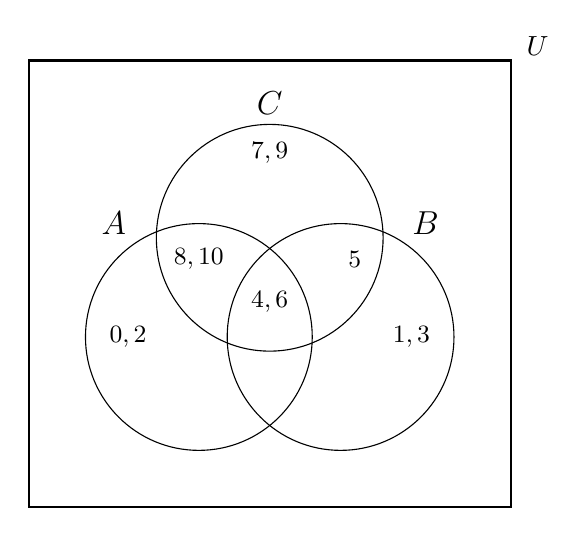
\begin{tikzpicture}[scale=0.9]
			      % Universe (a bit bigger so circles don't touch)
			      \draw[thick] (-3.4,-2.4) rectangle (3.4,3.9)
			      node[above right,xshift=2pt,yshift=-2pt] {$U$};

			      % Circle centres and radius
			      \def\r{1.6}
			      \coordinate (A) at (-1,0);
			      \coordinate (B) at ( 1,0);
			      \coordinate (C) at ( 0,1.4);

			      % Circles
			      \draw (A) circle (\r);
			      \draw (B) circle (\r);
			      \draw (C) circle (\r);

			      % Set labels
			      \node[font=\large] at (-2.2,1.6) {$A$};
			      \node[font=\large] at ( 2.2,1.6) {$B$};
			      \node[font=\large] at ( 0,3.3) {$C$};

			      % Region labels (slightly smaller font so they don't crowd)
			      \node[font=\small] at (-2.0,0)   {$0,2$};   % A only
			      \node[font=\small] at ( 2.0,0)   {$1,3$};   % B only
			      \node[font=\small] at ( 0,2.6)   {$7,9$};   % C only
			      \node[font=\small] at (-1.0,1.1) {$8,10$};  % A ∩ C only
			      \node[font=\small] at ( 1.2,1.1) {$5$};     % B ∩ C only
			      \node[font=\small] at ( 0,0.5)   {$4,6$};   % A ∩ B ∩ C
		      \end{tikzpicture}
	      \end{center}

	      %------------------------------------------------------------
	\item Suppose that $A$, $B$, and $C$ are sets such that $A \subseteq B$ and $B \subseteq C$.
	      Show that $A \subseteq C$.

	      \textbf{Proof.}
	      To show $A \subseteq C$, we must show that every element of $A$ is also an element of $C$.

	      Let $x$ be an arbitrary element of $A$. Since $A \subseteq B$, we have $x \in B$.
	      Since $B \subseteq C$, every element of $B$ is in $C$, so $x \in C$.

	      As $x$ was arbitrary in $A$, this shows $A \subseteq C$.
	      \hfill$\Box$

	      %------------------------------------------------------------
	\item Find the sets $A$ and $B$ if
	      \[
		      A \setminus B = \{1,5,7,8\},\quad
		      B \setminus A = \{2,10\},\quad
		      A \cap B = \{3,6,9\}.
	      \]

	      \textbf{Solution.}
	      The set $A$ is the disjoint union of the elements that are only in $A$ and those in $A \cap B$:
	      \[
		      A = (A \setminus B) \cup (A \cap B)
		      = \{1,5,7,8\} \cup \{3,6,9\}
		      = \{1,3,5,6,7,8,9\}.
	      \]
	      Similarly, $B$ consists of elements only in $B$ and those in $A \cap B$:
	      \[
		      B = (B \setminus A) \cup (A \cap B)
		      = \{2,10\} \cup \{3,6,9\}
		      = \{2,3,6,9,10\}.
	      \]

	      %------------------------------------------------------------
	\item Show that if $A$ and $B$ are sets, then $A \setminus B = A \cap B^{\mathrm{c}}$.

	      \textbf{Proof.}
	      We prove both inclusions.

	      \emph{($\subseteq$)}
	      Let $x \in A \setminus B$. By definition of set difference, $x \in A$ and $x \notin B$.
	      The statement $x \notin B$ means $x \in B^{\mathrm{c}}$.
	      Hence $x \in A$ and $x \in B^{\mathrm{c}}$, so $x \in A \cap B^{\mathrm{c}}$.

	      \emph{($\supseteq$)}
	      Let $x \in A \cap B^{\mathrm{c}}$. Then $x \in A$ and $x \in B^{\mathrm{c}}$, which means $x \notin B$.
	      Thus $x \in A$ and $x \notin B$, so $x \in A \setminus B$.

	      Since the two sets are subsets of each other, we conclude
	      \[
		      A \setminus B = A \cap B^{\mathrm{c}}.
	      \]
	      \hfill$\Box$

	      %------------------------------------------------------------
	\item What can you say about the sets $A$ and $B$ if we know that

	      \begin{enumerate}[label=(\alph*)]
		      \item $A \cup B = A$?

		            \textbf{Solution.}
		            If $A \cup B = A$, then adding $B$ does not introduce any new elements beyond those in $A$.
		            Formally, let $x \in B$. Then $x \in A \cup B = A$, so $x \in A$.
		            Therefore $B \subseteq A$.

		      \item $A \cap B = A$?

		            \textbf{Solution.}
		            If $A \cap B = A$, then intersecting with $B$ does not remove any elements from $A$.
		            Let $x \in A$. Then $x \in A \cap B$, so $x \in B$.
		            Hence $A \subseteq B$.

		      \item $A \setminus B = A$?

		            \textbf{Solution.}
		            Using $A \setminus B = A \cap B^{\mathrm{c}}$, we have
		            \[
			            A \cap B^{\mathrm{c}} = A.
		            \]
		            This means that every element of $A$ lies in $B^{\mathrm{c}}$, i.e. no element of $A$ lies in $B$.
		            So
		            \[
			            A \cap B = \emptyset,
		            \]
		            i.e. $A$ and $B$ are disjoint.

		      \item $A \cap B = B \cap A$?

		            \textbf{Solution.}
		            This holds for \emph{all} sets $A$ and $B$, since set intersection is commutative.
		            Therefore this condition does not give any additional information about $A$ and $B$.

		      \item $A \setminus B = B \setminus A$?

		            \textbf{Solution.}
		            Suppose $A \setminus B = B \setminus A$.

		            We first show $A \subseteq B$.
		            Let $x \in A$. If $x \notin B$, then $x \in A \setminus B$.
		            Since $A \setminus B = B \setminus A$, we also have $x \in B \setminus A$,
		            which implies $x \in B$ and $x \notin A$ — a contradiction.
		            Hence our assumption that $x \notin B$ is false, so $x \in B$.
		            Thus $A \subseteq B$.

		            Similarly, by symmetry, we can show $B \subseteq A$.

		            Therefore $A = B$.
	      \end{enumerate}

	      %------------------------------------------------------------
	\item In a group of $343$ employees in a company, the following information is known:
	      \begin{itemize}
		      \item $120$ employees are managers.
		      \item $135$ employees are engineers.
		      \item $80$ employees are in the sales department.
		      \item $50$ employees are both managers and engineers.
		      \item $30$ employees are both managers and in the sales department.
		      \item $25$ employees are both engineers and in the sales department.
		      \item $15$ employees are managers, engineers, and in the sales department.
	      \end{itemize}
	      How many employees are neither managers, engineers, nor in the sales department?
	      Draw a Venn diagram to show each of the sets and provide a brief explanation.

	      \textbf{Solution.}
	      Let $M$, $E$, and $S$ be the sets of managers, engineers, and salespeople respectively.
	      We are given:
	      \[
		      |M| = 120,\quad |E| = 135,\quad |S| = 80,
	      \]
	      \[
		      |M \cap E| = 50,\quad |M \cap S| = 30,\quad |E \cap S| = 25,\quad
		      |M \cap E \cap S| = 15.
	      \]

	      We first find the numbers in each of the $7$ non-empty regions of the three-set Venn diagram.

	      \begin{itemize}
		      \item Managers, engineers, and sales: $|M \cap E \cap S| = 15$.

		      \item Managers and engineers only (not sales):
		            \[
			            |M \cap E \text{ only}| = |M \cap E| - |M \cap E \cap S| = 50 - 15 = 35.
		            \]

		      \item Managers and sales only (not engineers):
		            \[
			            |M \cap S \text{ only}| = |M \cap S| - |M \cap E \cap S| = 30 - 15 = 15.
		            \]

		      \item Engineers and sales only (not managers):
		            \[
			            |E \cap S \text{ only}| = |E \cap S| - |M \cap E \cap S| = 25 - 15 = 10.
		            \]

		      \item Managers only (not engineers and not sales):
		            \[
			            |M \text{ only}| =
			            |M| - \bigl(|M \cap E \text{ only}| + |M \cap S \text{ only}| + |M \cap E \cap S|\bigr)
			            = 120 - (35 + 15 + 15) = 55.
		            \]

		      \item Engineers only:
		            \[
			            |E \text{ only}| =
			            |E| - \bigl(|M \cap E \text{ only}| + |E \cap S \text{ only}| + |M \cap E \cap S|\bigr)
			            = 135 - (35 + 10 + 15) = 75.
		            \]

		      \item Sales only:
		            \[
			            |S \text{ only}| =
			            |S| - \bigl(|M \cap S \text{ only}| + |E \cap S \text{ only}| + |M \cap E \cap S|\bigr)
			            = 80 - (15 + 10 + 15) = 40.
		            \]
	      \end{itemize}

	      The total number of employees in $M \cup E \cup S$ is
	      \begin{align*}
		      |M \cup E \cup S|
		       & = |M \text{ only}| + |E \text{ only}| + |S \text{ only}| \\
		       & + |M \cap E \text{ only}| + |M \cap S \text{ only}|      \\
		       & + |E \cap S \text{ only}| + |M \cap E \cap S|            \\
		       & = 55 + 75 + 40 + 35 + 15 + 10 + 15                       \\
		       & = 245.
	      \end{align*}
	      The total number of employees is $343$, so the number of employees who are
	      in none of the three sets (neither managers, engineers, nor sales) is
	      \[
		      343 - 245 = 98.
	      \]

	      \textbf{Answer:} $98$ employees are neither managers, engineers, nor in the sales department.

	      \medskip

	      \textbf{Venn diagram for $M$, $E$, and $S$.}

	      \begin{center}
		      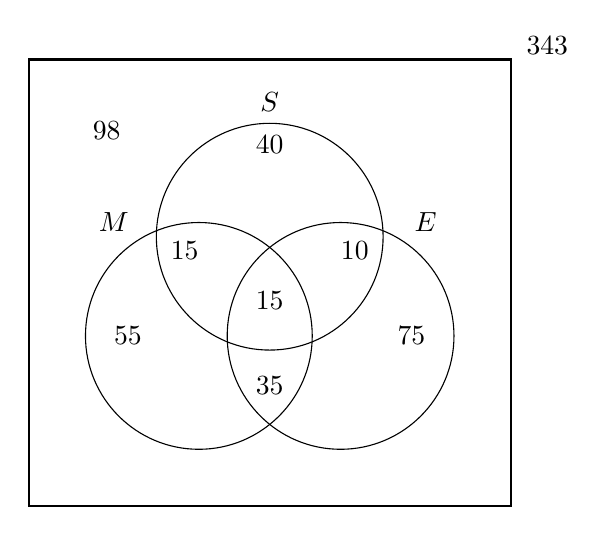
\begin{tikzpicture}[scale=0.9]
			      % Universe (total employees)
			      % \draw[thick] (-3,-2) rectangle (3,3) node[above right] {$343$};
			      \draw[thick] (-3.4,-2.4) rectangle (3.4,3.9)
			      node[above right,xshift=2pt,yshift=-2pt] {$343$};

			      % Circles
			      \def\M{(-1,0) circle (1.6)}
			      \def\E{(1,0) circle (1.6)}
			      \def\S{(0,1.4) circle (1.6)}

			      \draw \M;
			      \draw \E;
			      \draw \S;

			      \node at (-2.2,1.6) {$M$};
			      \node at (2.2,1.6) {$E$};
			      \node at (0,3.3) {$S$};

			      % Region counts
			      % M only
			      \node at (-2.0,0) {$55$};

			      % E only
			      \node at (2.0,0) {$75$};

			      % S only
			      \node at (0,2.7) {$40$};

			      % M ∩ E only
			      \node at (0,-0.7) {$35$};

			      % M ∩ S only
			      \node at (-1.2,1.2) {$15$};

			      % E ∩ S only
			      \node at (1.2,1.2) {$10$};

			      % M ∩ E ∩ S
			      \node at (0,0.5) {$15$};

			      % Outside all three
			      \node at (-2.3,2.9) {$98$};
		      \end{tikzpicture}
	      \end{center}

\end{enumerate}

\end{document}
